\documentclass[aspectratio=169,12pt]{beamer}
\usepackage[utf8]{inputenc}
\usepackage{amsmath, amssymb}
\usepackage{booktabs}
\usepackage{colortbl}
\usepackage{hyperref}
\usepackage{makecell}
\usepackage{ragged2e}
\usepackage{tikz}
\usetikzlibrary{arrows.meta, positioning, shapes.geometric, calc, tikzmark, shapes.misc, fit, decorations.pathreplacing}
\usepackage{tcolorbox}
\usepackage{array}
\usetheme{Madrid}

% Custom colors
\definecolor{correctgreen}{RGB}{0,150,0}
\definecolor{incorrectred}{RGB}{200,0,0}
\definecolor{counterblue}{RGB}{70,130,255}
\definecolor{highlightyellow}{RGB}{255,230,100}

\title{Branch Prediction}
\subtitle{Computer Architecture}
\author{Course 234267}
\date{}

\begin{document}

\frame{\titlepage}

%==========================================
\begin{frame}{2-Bit Counter Prediction (Threshold of 2)}
\vspace{-0.3cm}

% \begin{tikzpicture}[
%     every node/.style={font=\footnotesize},
%     pattern/.style={minimum width=0.5cm, minimum height=0.5cm, draw=black!60},
%     predict/.style={minimum width=0.5cm, minimum height=0.5cm, draw=black!60},
%     counter/.style={minimum width=0.5cm, minimum height=0.5cm, draw=counterblue, text=counterblue},
%     correct/.style={fill=correctgreen!20},
%     wrong/.style={fill=incorrectred!30},
%     arrow/.style={->, thick, >=stealth}
% ]

% % Labels
% \node[anchor=east] at (-0.5, 0) {\textbf{Pattern:}};
% \node[anchor=east] at (-0.5, -1) {\textbf{2-bit Prediction:}};
% \node[anchor=east] at (-0.5, -2) {\textbf{Counter:}};

% % Pattern row
% \foreach \i in {0,...,19} {
%     \pgfmathtruncatemacro{\val}{mod(\i,5) < 4 ? 1 : 0}
%     \pgfmathtruncatemacro{\groupnum}{floor(\i/5)}
%     \node[pattern, fill=\val ? white : gray!20] (p\i) at (\i*0.6, 0) {\val};
% }
% \node at (20*0.6, 0) {...};

\begin{tikzpicture}[
    every node/.style={font=\footnotesize},
    pattern/.style={minimum width=0.5cm, minimum height=0.5cm, draw=black!60},
    predict/.style={minimum width=0.5cm, minimum height=0.5cm, draw=black!60},
    counter/.style={minimum width=0.5cm, minimum height=0.5cm, draw=blue},
    correct/.style={fill=green!20},
    wrong/.style={fill=red!30},
    arrow/.style={->, thick, >=stealth}
]

% Labels
\node[anchor=east] at (-0.5, 0) {\textbf{Pattern:}};
\node[anchor=east] at (-0.5, -1) {\textbf{2-bit Prediction:}};
\node[anchor=east] at (-0.5, -2) {\textbf{Counter:}};

% Pattern row
\foreach \i in {0,...,19} {
    \pgfmathtruncatemacro{\val}{mod(\i,5) < 4 ? 1 : 0}
    \pgfmathtruncatemacro{\groupnum}{floor(\i/5)}
    \ifnum\val=1
        \node[pattern, fill=white] (p\i) at (\i*0.6, 0) {\val};
    \else
        \node[pattern, fill=gray!20] (p\i) at (\i*0.6, 0) {\val};
    \fi
}
\node at (20*0.6, 0) {...};

% Prediction row
\pause
\foreach \i in {0,...,19} {
    \node[predict] (pred\i) at (\i*0.6, -1) {1};
}
\node at (20*0.6, -1) {...};

% Counter row
\pause
\foreach \i in {0,...,19} {
    \pgfmathtruncatemacro{\posInGroup}{mod(\i,5)}
    \ifnum\posInGroup=0
        \node[counter, color=blue] (c\i) at (\i*0.6, -2) {2};
    \else
        \ifnum\posInGroup=4
            \node[counter, color=blue] (c\i) at (\i*0.6, -2) {2};
        \else
            \node[counter, color=blue] (c\i) at (\i*0.6, -2) {3};
        \fi
    \fi
}
\node at (20*0.6, -2) {2 3 ...};

% Misprediction indicators
\pause
\foreach \i in {4,9,14,19} {
    % Highlight mispredicted positions
    \node[predict, wrong] at (\i*0.6, -1) {1};
    \draw[red, ultra thick] (p\i.south west) -- (p\i.south east);
    \draw[red, ultra thick] (pred\i.north west) -- (pred\i.north east);
    
    % Add X mark for misprediction
    \node[color=red, font=\Large] at (\i*0.6, -0.5) {$\times$};
}
% Correct prediction indicators (check marks)
\pause
\foreach \i in {0,1,2,3,5,6,7,8,10,11,12,13,15,16,17,18} {
    \node[color=green!60!black, font=\small] at (\i*0.6, -0.5) {$\checkmark$};
}
% Group brackets
\pause
\foreach \g in {0,1,2,3} {
    \pgfmathtruncatemacro{\startx}{\g*5}
    \pgfmathtruncatemacro{\endx}{\g*5+4}
    \pgfmathtruncatemacro{\gnum}{\g+1}
    \draw[decoration={brace,amplitude=5pt,mirror}, decorate, thick, gray] 
        (\startx*0.6-0.25, -2.5) -- (\endx*0.6+0.25, -2.5);
    \node[gray] at (\startx*0.6+1.2, -2.9) {iteration \gnum};
}

\end{tikzpicture}

\vspace{0.3cm}
\pause
\begin{alertblock}{Key Observation}
\centering
\textcolor{incorrectred}{\textbf{2-bit counter $\rightarrow$ one misprediction every iteration}}
\end{alertblock}

\pause
\vspace{0.2cm}
\begin{block}{Performance Example}
\begin{columns}[T]
\column{0.55\textwidth}
\begin{itemize}
\item<8-> Assume 1 of 20 branches mispredicts\\
      \textcolor{gray}{\small (19 predictions are correct)}
\item<9-> Branch frequency: 20\%\\
      \textcolor{gray}{\small (1 of 5 instructions is branch)}
\item<10-> \textcolor{incorrectred}{\textbf{$\rightarrow$ 1 mispredict every 100 instructions}}
\end{itemize}

\column{0.45\textwidth}
\begin{itemize}
\item<11-> IPC without penalty = 2\\
      \textcolor{gray}{\small (two instructions finish per cycle)}
\item<12-> Mispredict penalty: 10 cycles
\item<13-> \textcolor{incorrectred}{\textbf{$\rightarrow$ 1 mispredict every 50 cycles}}
\item<14-> \textcolor{incorrectred}{\textbf{$\rightarrow$ 10 cycles penalty every 50 cycles}}
\end{itemize}
\end{columns}

\vspace{0.3cm}
\visible<15->{
\begin{tcolorbox}[colback=red!10, colframe=red!60, boxrule=2pt]
\centering
\Large \textcolor{incorrectred}{\textbf{$\rightarrow$ 20\% performance loss!}}
\end{tcolorbox}
}
\end{block}

\end{frame}

\begin{frame}{Better Idea: Use Branch History}

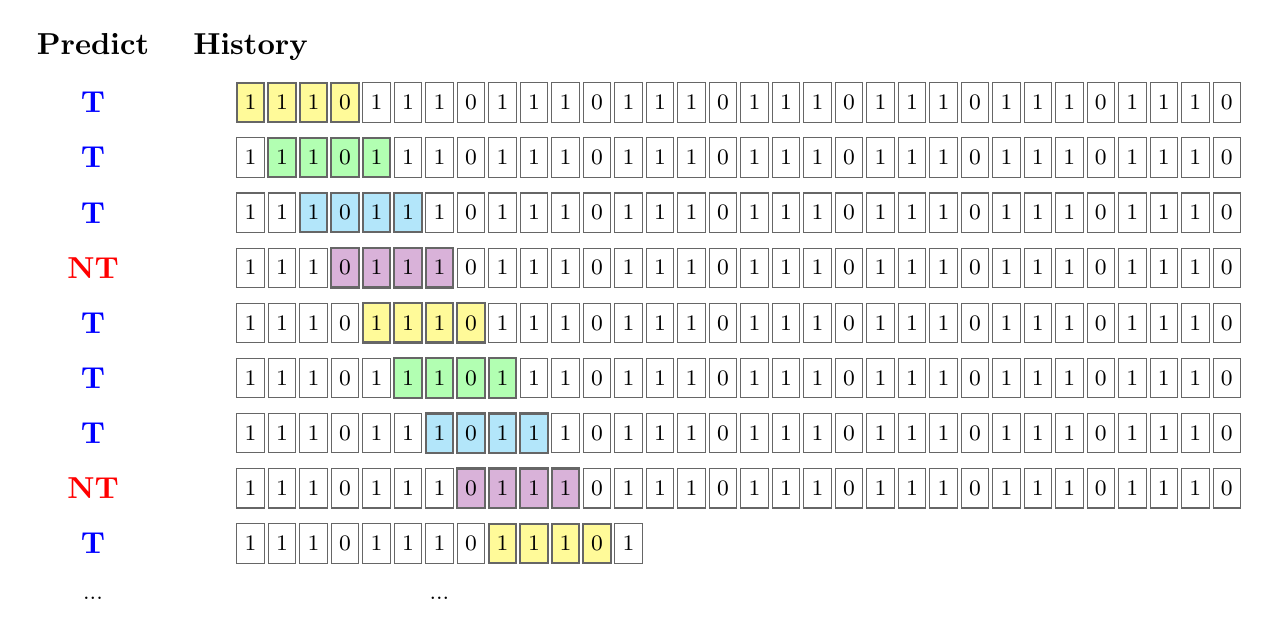
\begin{tikzpicture}[
    every node/.style={font=\footnotesize},
    bit/.style={minimum width=0.35cm, minimum height=0.5cm, inner sep=1pt, draw=black!60},
    history1110/.style={bit, fill=yellow!40, thick},
    history1101/.style={bit, fill=green!30, thick},
    history1011/.style={bit, fill=cyan!30, thick},
    history0111/.style={bit, fill=violet!30, thick},
    predict/.style={font=\fontsize{11}{13}\selectfont\bfseries, minimum width=1cm},
    label/.style={font=\fontsize{11}{13}\selectfont\bfseries}
]

% Labels positioned using relative positioning
\node[label, text height=1.5ex, text depth=.25ex] (predict_label) at (0, 0) {Predict};
\node[label, text height=1.5ex, text depth=.25ex] (history_label) at (2, 0) {History};

% Pattern template (repeated pattern: 11101110...)
\def\patternseq{1,1,1,0,1,1,1,0,1,1,1,0,1,1,1,0,1,1,1,0,1,1,1,0,1,1,1,0,1,1,1,0}

% Define row spacing
\def\rowspacing{0.7}

% Row 1 - History: 1110 -> Predict T
\node[predict, text=blue] (pred1) at (0, -1*\rowspacing) {T};
\foreach \i in {0,...,31} {
    \pgfmathparse{{\patternseq}[\i]}
    \pgfmathtruncatemacro{\val}{\pgfmathresult}
    \ifnum\i<4
        \node[history1110] at (2 + \i*0.4, -1*\rowspacing) {\val};
    \else
        \node[bit] at (2 + \i*0.4, -1*\rowspacing) {\val};
    \fi
}

% Row 2 - History: 1101 -> Predict T
\node[predict, text=blue] (pred2) at (0, -2*\rowspacing) {T};
\foreach \i in {0,...,31} {
    \pgfmathparse{{\patternseq}[\i]}
    \pgfmathtruncatemacro{\val}{\pgfmathresult}
    \ifnum\i>0 \ifnum\i<5
        \node[history1101] at (2 + \i*0.4, -2*\rowspacing) {\val};
    \else
        \node[bit] at (2 + \i*0.4, -2*\rowspacing) {\val};
    \fi \fi
    \ifnum\i=0
        \node[bit] at (2 + \i*0.4, -2*\rowspacing) {\val};
    \fi
}

% Row 3 - History: 1011 -> Predict T  
\node[predict, text=blue] (pred3) at (0, -3*\rowspacing) {T};
\foreach \i in {0,...,31} {
    \pgfmathparse{{\patternseq}[\i]}
    \pgfmathtruncatemacro{\val}{\pgfmathresult}
    \ifnum\i>1 \ifnum\i<6
        \node[history1011] at (2 + \i*0.4, -3*\rowspacing) {\val};
    \else
        \node[bit] at (2 + \i*0.4, -3*\rowspacing) {\val};
    \fi \fi
    \ifnum\i<2
        \node[bit] at (2 + \i*0.4, -3*\rowspacing) {\val};
    \fi
}

% Row 4 - History: 0111 -> Predict NT
\node[predict, text=red] (pred4) at (0, -4*\rowspacing) {NT};
\foreach \i in {0,...,31} {
    \pgfmathparse{{\patternseq}[\i]}
    \pgfmathtruncatemacro{\val}{\pgfmathresult}
    \ifnum\i>2 \ifnum\i<7
        \node[history0111] at (2 + \i*0.4, -4*\rowspacing) {\val};
    \else
        \node[bit] at (2 + \i*0.4, -4*\rowspacing) {\val};
    \fi \fi
    \ifnum\i<3
        \node[bit] at (2 + \i*0.4, -4*\rowspacing) {\val};
    \fi
}

% Row 5 - History: 1110 -> Predict T
\node[predict, text=blue] (pred5) at (0, -5*\rowspacing) {T};
\foreach \i in {0,...,31} {
    \pgfmathparse{{\patternseq}[\i]}
    \pgfmathtruncatemacro{\val}{\pgfmathresult}
    \ifnum\i>3 \ifnum\i<8
        \node[history1110] at (2 + \i*0.4, -5*\rowspacing) {\val};
    \else
        \node[bit] at (2 + \i*0.4, -5*\rowspacing) {\val};
    \fi \fi
    \ifnum\i<4
        \node[bit] at (2 + \i*0.4, -5*\rowspacing) {\val};
    \fi
}

% Row 6 - History: 1101 -> Predict T
\node[predict, text=blue] (pred6) at (0, -6*\rowspacing) {T};
\foreach \i in {0,...,31} {
    \pgfmathparse{{\patternseq}[\i]}
    \pgfmathtruncatemacro{\val}{\pgfmathresult}
    \ifnum\i>4 \ifnum\i<9
        \node[history1101] at (2 + \i*0.4, -6*\rowspacing) {\val};
    \else
        \node[bit] at (2 + \i*0.4, -6*\rowspacing) {\val};
    \fi \fi
    \ifnum\i<5
        \node[bit] at (2 + \i*0.4, -6*\rowspacing) {\val};
    \fi
}

% Row 7 - History: 1011 -> Predict T
\node[predict, text=blue] (pred7) at (0, -7*\rowspacing) {T};
\foreach \i in {0,...,31} {
    \pgfmathparse{{\patternseq}[\i]}
    \pgfmathtruncatemacro{\val}{\pgfmathresult}
    \ifnum\i>5 \ifnum\i<10
        \node[history1011] at (2 + \i*0.4, -7*\rowspacing) {\val};
    \else
        \node[bit] at (2 + \i*0.4, -7*\rowspacing) {\val};
    \fi \fi
    \ifnum\i<6
        \node[bit] at (2 + \i*0.4, -7*\rowspacing) {\val};
    \fi
}

% Row 8 - History: 0111 -> Predict NT
\node[predict, text=red] (pred8) at (0, -8*\rowspacing) {NT};
\foreach \i in {0,...,31} {
    \pgfmathparse{{\patternseq}[\i]}
    \pgfmathtruncatemacro{\val}{\pgfmathresult}
    \ifnum\i>6 \ifnum\i<11
        \node[history0111] at (2 + \i*0.4, -8*\rowspacing) {\val};
    \else
        \node[bit] at (2 + \i*0.4, -8*\rowspacing) {\val};
    \fi \fi
    \ifnum\i<7
        \node[bit] at (2 + \i*0.4, -8*\rowspacing) {\val};
    \fi
}

% Row 9 - History: 1110 -> Predict T
\node[predict, text=blue] (pred9) at (0, -9*\rowspacing) {T};
\foreach \i in {0,...,12} {
    \pgfmathparse{{\patternseq}[\i]}
    \pgfmathtruncatemacro{\val}{\pgfmathresult}
    \ifnum\i>7 \ifnum\i<12
        \node[history1110] at (2 + \i*0.4, -9*\rowspacing) {\val};
    \else
        \node[bit] at (2 + \i*0.4, -9*\rowspacing) {\val};
    \fi \fi
    \ifnum\i<8
        \node[bit] at (2 + \i*0.4, -9*\rowspacing) {\val};
    \fi
}

% ... dots
\node at (0, -10*\rowspacing) {...};
\node at (2 + 6*0.4, -10*\rowspacing) {...};

\end{tikzpicture}

\end{frame}

%==========================================
\definecolor{correctgreen}{RGB}{0,150,0}
\definecolor{incorrectred}{RGB}{200,0,0}
\definecolor{counterblue}{RGB}{70,130,255}
\definecolor{highlightyellow}{RGB}{255,230,100}
\definecolor{codeblue}{RGB}{0,0,200}

% Command to highlight state changes
\newcommand{\stateHighlight}[2]{%
  \ifnum#1=1
    \cellcolor{highlightyellow}#2%
  \else
    #2%
  \fi
}

% Macro for BHR display as boxes
\newcommand{\BHRbox}[4]{%
  \begin{tikzpicture}[baseline=(current bounding box.center)]
    \foreach \bit [count=\i] in {#1,#2,#3,#4} {
      \node[draw, minimum width=6mm, minimum height=5mm, inner sep=1pt] at (\i*0.7,0) {\footnotesize\bit};
    }
  \end{tikzpicture}
}

% Main frame macro for Local History Predictor
\newcommand{\localFrame}[9]{%
  % #1: Branch outcome text
  % #2: IP1 BHR (format: {b1}{b2}{b3}{b4})
  % #3: IP2 BHR
  % #4: IP3 BHR
  % #5: r1 value
  % #6: r2 value
  % #7: r3 value
  % #8: State table changes (format: index,state)
  % #9: Result description
  \begin{frame}
    \frametitle{Local History Branch Predictor}
    \begin{columns}[T]
      \column{0.30\textwidth}
      \begin{tcolorbox}[colback=gray!5, colframe=gray!50, boxrule=0.5pt, left=2pt, right=2pt, top=2pt, bottom=2pt]
        \footnotesize\ttfamily
        \begin{tabbing}
        \hspace{2em}\=\hspace{2em}\=\kill
        \> Addi r5, r0, 5\\
        \> Addi r1, r0, 100\\
        L1:\> Addi r2, r0, 2\\
        L2:\> Mod r3, r1, r2\\
        \> Bne r3, r0, IF\\
        \> . . .\\
        IF:\> Addi r2, r2, 1\\
        \> Bne r2, r5, L2\\
        \> Subi r1, r1, 1\\
        \> Bne r1, r0, L1
        \end{tabbing}
      \end{tcolorbox}
      
      \vspace{0.5em}
      \centering
      \colorbox{highlightyellow}{\textbf{#1}}
      
      \column{0.70\textwidth}
      \footnotesize
      \begin{tabular}{|c|ccc|c}
        \toprule
        tag & \multicolumn{4}{c|}{BHRs} \\
        \midrule
        IP1 & \multicolumn{4}{c|}{\BHRbox#2} \\
        IP2 & \multicolumn{4}{c|}{\BHRbox#3} \\
        IP3 & \multicolumn{4}{c|}{\BHRbox#4} \\
        \bottomrule
      \end{tabular}
      
      \vspace{0.8em}
      \begin{columns}
        \column{0.35\textwidth}
        \centering
        \begin{tabular}{c|r}
          \toprule
          Reg & Value \\
          \midrule
          r1 & #5 \\
          r2 & #6 \\
          r3 & #7 \\
          \bottomrule
        \end{tabular}
        
        \column{0.65\textwidth}
        \centering\tiny
        \stateTable{#8}
      \end{columns}
      
      \vspace{0.5em}
      \centering
      \textcolor{blue}{\small #9}
    \end{columns}
  \end{frame}
}

% Main frame macro for Global History Predictor
\newcommand{\globalFrame}[7]{%
  % #1: Branch outcome text
  % #2: Global BHR (format: {b1}{b2}{b3}{b4})
  % #3: r1 value
  % #4: r2 value
  % #5: r3 value
  % #6: State table changes (format: index,state)
  % #7: Result description
  \begin{frame}
    \frametitle{Global History Branch Predictor}
    \begin{columns}[T]
      \column{0.42\textwidth}
      \begin{tcolorbox}[colback=gray!5, colframe=gray!50, boxrule=0.5pt, left=2pt, right=2pt, top=2pt, bottom=2pt]
        \footnotesize\ttfamily
        \begin{tabbing}
        \hspace{2em}\=\hspace{2em}\=\kill
        \> Addi r5, r0, 5\\
        \> Addi r1, r0, 100\\
        L1:\> Addi r2, r0, 2\\
        \> Mod r3, r1, r2\\
        L2:\> Bne r3, r0, IF\\
        \> . . .\\
        IF:\> Addi r2, r2, 1\\
        \> Bne r2, r5, L2\\
        \> Subi r1, r1, 1\\
        \> Bne r1, r0, L1
        \end{tabbing}
      \end{tcolorbox}
      
      \vspace{0.5em}
      \centering
      \colorbox{highlightyellow}{\textbf{#1}}
      
      \column{0.58\textwidth}
      \footnotesize
      \begin{center}
        \textbf{Global BHR}\\[0.3em]
        \BHRbox#2
      \end{center}
      
      \vspace{0.8em}
      \begin{columns}
        \column{0.35\textwidth}
        \centering
        \begin{tabular}{c|r}
          \toprule
          Reg & Value \\
          \midrule
          r1 & #3 \\
          r2 & #4 \\
          r3 & #5 \\
          \bottomrule
        \end{tabular}
        
        \column{0.65\textwidth}
        \centering
        \textbf{Global Table}\\[0.3em]
        \tiny
        \stateTable{#6}
      \end{columns}
      
      \vspace{0.5em}
      \centering
      \textcolor{blue}{\small #7}
    \end{columns}
  \end{frame}
}

% State table macro
\newcommand{\stateTable}[1]{%
  % #1: comma-separated list of index:state:highlight
  % Format: 0:WT:0,3:ST:1,12:WNT:0,...
  \begin{tabular}{c|c||c|c}
    \toprule
    \multicolumn{2}{c||}{States 0-7} & \multicolumn{2}{c}{States 8-15} \\
    \midrule
    \stateRow{0}{#1} & \stateRow{8}{#1} \\
    \stateRow{1}{#1} & \stateRow{9}{#1} \\
    \stateRow{2}{#1} & \stateRow{10}{#1} \\
    \stateRow{3}{#1} & \stateRow{11}{#1} \\
    \stateRow{4}{#1} & \stateRow{12}{#1} \\
    \stateRow{5}{#1} & \stateRow{13}{#1} \\
    \stateRow{6}{#1} & \stateRow{14}{#1} \\
    \stateRow{7}{#1} & \stateRow{15}{#1} \\
    \bottomrule
  \end{tabular}
}

% Helper to format state with color
\newcommand{\formatState}[1]{%
  \ifnum\pdfstrcmp{#1}{ST}=0\textcolor{correctgreen}{\textbf{#1}}%
  \else\ifnum\pdfstrcmp{#1}{WT}=0#1%
  \else\ifnum\pdfstrcmp{#1}{WNT}=0\textcolor{incorrectred}{#1}%
  \else\ifnum\pdfstrcmp{#1}{SNT}=0\textcolor{incorrectred}{\textbf{#1}}%
  \else #1%
  \fi\fi\fi\fi%
}

% Helper to get state for specific index
\newcommand{\stateRow}[2]{%
  % #1: index, #2: full state string
  % Returns the row for this index
  #1 & \getStateForIndex{#1}{#2}%
}

% Parse state string and return formatted state for given index
\newcommand{\getStateForIndex}[2]{%
  % Default all to WT, then override based on input
  \def\tempstate{WT}%
  \def\temphighlight{0}%
  % Parse the input string for this index
  \parseStateString{#1}{#2}%
  \ifnum\temphighlight=1
    \cellcolor{highlightyellow}\formatState{\tempstate}%
  \else
    \formatState{\tempstate}%
  \fi
}

% Helper to parse state string - simplified version
\newcommand{\parseStateString}[2]{%
  % This is a simplified implementation
  % In practice, you'd parse #2 to find if #1 appears
  % For now, using manual specification in frames
}

% Advanced macro for complete state specification
% Usage: \fullStateTable{index1/state1/highlight1,index2/state2/highlight2,...}
\newcommand{\fullStateTable}[1]{%
  \def\stateZero{WT}\def\highlightZero{0}%
  \def\stateOne{WT}\def\highlightOne{0}%
  \def\stateTwo{WT}\def\highlightTwo{0}%
  \def\stateThree{WT}\def\highlightThree{0}%
  \def\stateFour{WT}\def\highlightFour{0}%
  \def\stateFive{WT}\def\highlightFive{0}%
  \def\stateSix{WT}\def\highlightSix{0}%
  \def\stateSeven{WT}\def\highlightSeven{0}%
  \def\stateEight{WT}\def\highlightEight{0}%
  \def\stateNine{WT}\def\highlightNine{0}%
  \def\stateTen{WT}\def\highlightTen{0}%
  \def\stateEleven{WT}\def\highlightEleven{0}%
  \def\stateTwelve{WT}\def\highlightTwelve{0}%
  \def\stateThirteen{WT}\def\highlightThirteen{0}%
  \def\stateFourteen{WT}\def\highlightFourteen{0}%
  \def\stateFifteen{WT}\def\highlightFifteen{0}%
  % Parse input and update states
  % For demonstration, manually setting based on frame
  \begin{tabular}{c|c||c|c}
    \toprule
    \multicolumn{2}{c||}{States 0-7} & \multicolumn{2}{c}{States 8-15} \\
    \midrule
    0 & \ifnum\highlightZero=1\cellcolor{highlightyellow}\fi\formatState{\stateZero} & 
    8 & \ifnum\highlightEight=1\cellcolor{highlightyellow}\fi\formatState{\stateEight} \\
    1 & \ifnum\highlightOne=1\cellcolor{highlightyellow}\fi\formatState{\stateOne} & 
    9 & \ifnum\highlightNine=1\cellcolor{highlightyellow}\fi\formatState{\stateNine} \\
    2 & \ifnum\highlightTwo=1\cellcolor{highlightyellow}\fi\formatState{\stateTwo} & 
    10 & \ifnum\highlightTen=1\cellcolor{highlightyellow}\fi\formatState{\stateTen} \\
    3 & \ifnum\highlightThree=1\cellcolor{highlightyellow}\fi\formatState{\stateThree} & 
    11 & \ifnum\highlightEleven=1\cellcolor{highlightyellow}\fi\formatState{\stateEleven} \\
    4 & \ifnum\highlightFour=1\cellcolor{highlightyellow}\fi\formatState{\stateFour} & 
    12 & \ifnum\highlightTwelve=1\cellcolor{highlightyellow}\fi\formatState{\stateTwelve} \\
    5 & \ifnum\highlightFive=1\cellcolor{highlightyellow}\fi\formatState{\stateFive} & 
    13 & \ifnum\highlightThirteen=1\cellcolor{highlightyellow}\fi\formatState{\stateThirteen} \\
    6 & \ifnum\highlightSix=1\cellcolor{highlightyellow}\fi\formatState{\stateSix} & 
    14 & \ifnum\highlightFourteen=1\cellcolor{highlightyellow}\fi\formatState{\stateFourteen} \\
    7 & \ifnum\highlightSeven=1\cellcolor{highlightyellow}\fi\formatState{\stateSeven} & 
    15 & \ifnum\highlightFifteen=1\cellcolor{highlightyellow}\fi\formatState{\stateFifteen} \\
    \bottomrule
  \end{tabular}
}

\section{Local History Branch Predictor}

% Local History Predictor Frames
\localFrame{Not Taken}{{0}{0}{0}{0}}{{0}{0}{0}{0}}{{0}{0}{0}{0}}{100}{2}{0}{0:WT:0}{Initial state}

\localFrame{Not Taken}{{0}{0}{0}{0}}{{0}{0}{0}{0}}{{0}{0}{0}{0}}{100}{2}{0}{0:WNT:1}{Misprediction (predicted taken, was not taken)}

\localFrame{Taken}{{0}{0}{0}{0}}{{0}{0}{0}{0}}{{0}{0}{0}{0}}{100}{3}{0}{0:WT:1}{State update}

\localFrame{Taken}{{0}{0}{0}{0}}{{0}{0}{0}{1}}{{0}{0}{0}{0}}{100}{3}{0}{0:ST:1}{Correct prediction}

\localFrame{Taken}{{0}{0}{0}{0}}{{0}{0}{0}{1}}{{0}{0}{0}{0}}{100}{3}{1}{0:WNT:0}{State update}

\localFrame{Taken}{{0}{0}{0}{1}}{{0}{0}{0}{1}}{{0}{0}{0}{0}}{100}{3}{1}{0:WT:1}{Misprediction}

\localFrame{Taken}{{0}{0}{0}{1}}{{0}{0}{0}{1}}{{0}{0}{0}{0}}{100}{4}{1}{0:ST:1}{Correct prediction}

\localFrame{Taken}{{0}{0}{0}{1}}{{0}{0}{1}{1}}{{0}{0}{0}{0}}{100}{4}{1}{0:ST:1}{Correct prediction}

\localFrame{Not Taken}{{0}{0}{0}{1}}{{0}{0}{1}{1}}{{0}{0}{0}{0}}{100}{4}{0}{0:ST:0}{State update}

\localFrame{Not Taken}{{0}{0}{1}{0}}{{0}{0}{1}{1}}{{0}{0}{0}{0}}{100}{4}{0}{0:WNT:1}{Misprediction}

\localFrame{Not Taken}{{0}{0}{1}{0}}{{0}{0}{1}{1}}{{0}{0}{0}{0}}{100}{5}{0}{0:ST:1,3:ST:0}{State update}

\localFrame{Not Taken}{{0}{0}{1}{0}}{{0}{1}{1}{0}}{{0}{0}{0}{0}}{100}{5}{0}{3:WNT:1}{Misprediction}

\localFrame{Taken}{{0}{0}{1}{0}}{{0}{1}{1}{0}}{{0}{0}{0}{0}}{99}{5}{0}{0:ST:0}{State update}

\localFrame{Taken}{{0}{0}{1}{0}}{{0}{1}{1}{0}}{{0}{0}{0}{1}}{99}{5}{0}{0:ST:1}{Correct prediction}

% Transition slide
\begin{frame}
  \frametitle{Global History Predictor}
  \begin{center}
    \Large Now switching to \textbf{Global BHR}
  \end{center}
  
  \vspace{1em}
  
  \begin{itemize}
    \item Using a single global BHR table
    \item In contrast to local predictors (each IP has own BHR and state table)
    \item Still tracking history of 4 branches (4-bit BHR)
  \end{itemize}
  
  \vspace{1em}
  
  \begin{tcolorbox}[colback=blue!10, colframe=blue!50, width=0.8\textwidth]
    \centering
    \textbf{Predictor Size Calculation}\\[0.5em]
    Predictor size = $\text{history\_size} + 2 \times 2^{\text{history\_size}}$\\[0.3em]
    With history\_size = 4:\\
    Predictor size = $4 + 2 \times 2^4 = 36$ bits\\[0.3em]
    \textcolor{correctgreen}{vs. 66KB for local history/state arrays!}
  \end{tcolorbox}
\end{frame}

% Global History Predictor Frames
\globalFrame{Not Taken}{{0}{0}{0}{0}}{100}{2}{0}{0:WT:0}{Global BHR - Initial state}

\globalFrame{Not Taken}{{0}{0}{0}{0}}{100}{2}{0}{0:WNT:1}{Misprediction (predicted taken, was not taken)}

\globalFrame{Taken}{{0}{0}{0}{0}}{100}{3}{0}{0:WNT:0}{State update}

\globalFrame{Taken}{{0}{0}{0}{1}}{100}{3}{0}{0:WT:1}{Misprediction}

\globalFrame{Taken}{{0}{0}{0}{1}}{100}{3}{1}{0:WT:0}{State update}

\globalFrame{Taken}{{0}{0}{1}{1}}{100}{3}{1}{3:ST:1}{Correct prediction}

\globalFrame{Taken}{{0}{0}{1}{1}}{100}{4}{1}{3:ST:0}{State update}

\globalFrame{Taken}{{0}{1}{1}{1}}{100}{4}{1}{3:ST:1}{Correct prediction}

\globalFrame{Not Taken}{{0}{1}{1}{1}}{100}{4}{0}{3:ST:0}{State update}

\globalFrame{Not Taken}{{1}{1}{1}{0}}{100}{4}{0}{14:WNT:1}{Misprediction}

\globalFrame{Not Taken}{{1}{1}{1}{0}}{100}{5}{0}{14:WNT:0}{State update}

\globalFrame{Not Taken}{{1}{1}{0}{0}}{100}{5}{0}{12:WNT:1}{Misprediction}

\globalFrame{Taken}{{1}{1}{0}{0}}{99}{5}{0}{12:WT:0}{State update}

\globalFrame{Taken}{{1}{0}{0}{1}}{99}{5}{0}{12:ST:1}{Correct prediction}

%==========================================
% Add more slides here as needed

\end{document}